%\begin{figure}[htb]
\begin{teaserfigure}
  \centering
  \subfloat[scene representation]{
    \label{fig:teaser:scene}
    % 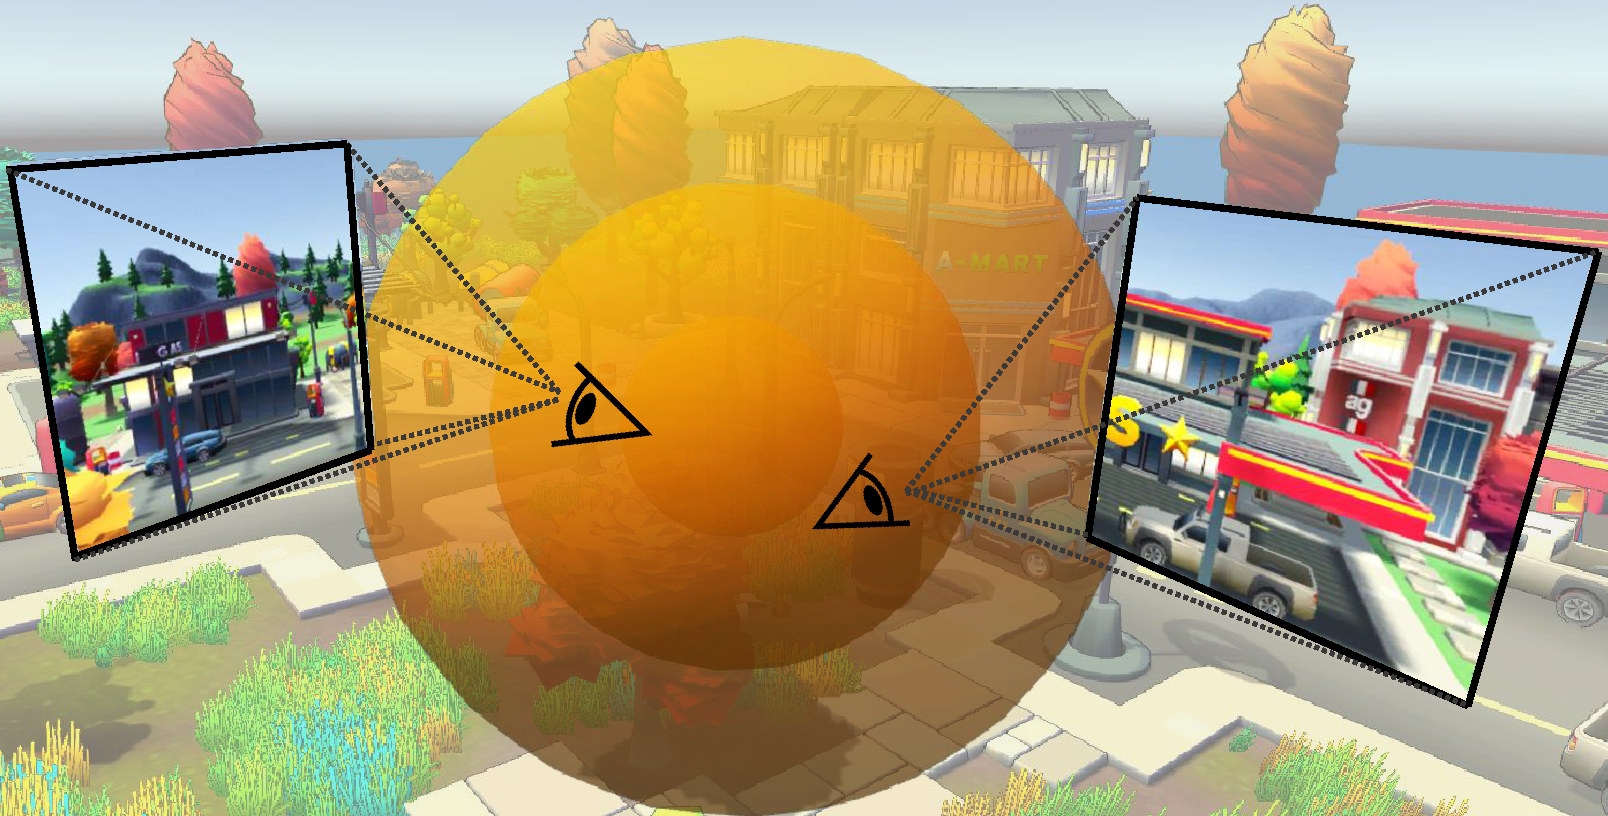
\includegraphics[height=4.5cm]{TOG/figs/scene.pdf}
    \includegraphics[trim=100 0 120 0,clip,height=5.5cm]{TOG/figs/teaser/teaser_1a_wc.pdf}
  }%subfloat
  \subfloat[overall quality]{
    \label{fig:teaser:latency}
    % \includegraphics[height=4.5cm]{TOG/figs/teaser_1b_update.pdf}
    % text version
    % \includegraphics[height=5.5cm]{TOG/figs/teaser/overall_crop_zh_large.pdf}
    % color version
    \includegraphics[height=5.5cm]{TOG/figs/teaser/overall_crop_color_s.pdf}
    % nerf: 15+s/per infer
  }%subfloat
  \subfloat[foveal quality]{
    \label{fig:teaser:quality}
    % 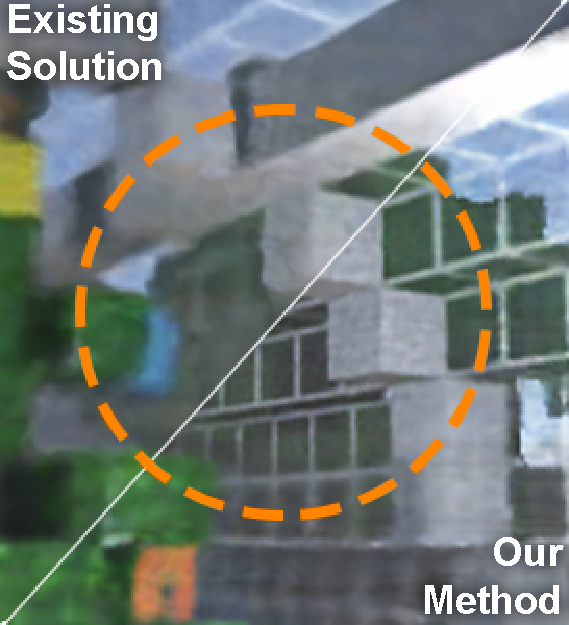
\includegraphics[height=4.5cm]{TOG/figs/teaser_1c.pdf}
    % text version
    % \includegraphics[height=5.5cm]{TOG/figs/teaser/overall_flat_zh_large.pdf}
    % color version
    \includegraphics[height=5.5cm]{TOG/figs/teaser/overall_flat_color_s.pdf}
  }%subfloat
 \Caption{Illustration of our gaze-contingent neural synthesis method.}
 {% 
\subref{fig:teaser:scene} Visualization of our active-viewing-tailored egocentric neural scene representation.
\subref{fig:teaser:latency} Our method allows for extremely low data storage of high-quality 3D scene assets and achieves high perceptual image quality and low latency for interactive virtual reality. Here, we compare our method with the state-of-the-art alternative neural synthesis \protect\cite{mildenhall2020nerf} and foveated rendering solutions \cite{perry2002gaze,Patney:2016:TFR} and demonstrate that our method significantly reduces more than $99\%$ time consumption (from 9s to 20ms) and data storage (from 100MB mesh to 0.5MB neural model) for first-person immersive viewing. The orange circle indicates the viewer's gaze position. We also show zoomed-in views of the foveal images generated by various methods in \subref{fig:teaser:quality} and show that our method is superior compared to existing methods in achieving high perceptual image fidelity.%\qisun{The quality of Nerf is super invisible in this design to me. @Zhenyi, let's flip Nerf and F-GT.}
%\qisun{(Jan 24, 2021) Let's add some latency numbers to
%\zh{15s/infer for NeRF}\subref{fig:teaser:latency}?}
%\qisun{(Jan 25) Can I get your help on adding the numbers with the fancy font to the figures directly in \subref{fig:teaser:latency}?}
 }
 \label{fig:teaser}
%\end{figure}
\end{teaserfigure}
